\documentclass[12pt, a4paper]{article}
\usepackage[utf8]{inputenc}
\usepackage[russian]{babel}
\usepackage[pdftex]{graphicx, color}
\usepackage{amsmath}
\usepackage{amsfonts}
\usepackage{amssymb}
\usepackage{amsthm}
\usepackage[left=2cm,right=1.5cm,top=1.5cm,bottom=2cm]{geometry}
\usepackage{indentfirst}
\usepackage{hyperref}


\usepackage{setspace}
\onehalfspacing
\graphicspath{{pic/}}

\begin{document}

    \thispagestyle{empty}

    \begin{singlespace}
    \begin{titlepage}
        \begin{center}
            
\includegraphics[height = 3cm]{msu.png}

            {\scshape Московский государственный университет имени М.~В.~Ломоносова}\\
            Факультет вычислительной математики и кибернетики\\
            \centerline{\hfill\hrulefill\hrulefill\hrulefill\hrulefill\hfill}

            \vfill

            {\LARGE Отчет о проделанной работе на соревновании на Kaggle: Предсказание зарплаты по тексту объявления}

            \vspace{1cm}

        \end{center}

        \vfill
        \begin{flushright}
            \textit{Студент 3 курса ВМК (317 группа):}\\
                Оспанов А.М.

            \vspace{5mm}

        \end{flushright}

        \vfill

        \begin{center}
        Москва, 2015
        \end{center}
    \end{titlepage}
    \end{singlespace}

    \tableofcontents

    \newpage
    \section{Выделение признаков}
        Как и в любой задаче машинного обучения, нам нужно выделить признаки из исходных данных и представить их в некотором виде для дальнейшей работы. При решении данной задачи были перепробованы разные способы представления данных для обучения. Но хорошо заработал только самый первый придуманный вариант (ирония?).

        Для обработки данных использовалась библиотека nltk (\url{http://www.nltk.org/}), а именно: модуль выделения токенов (nltk.tokenize), список стоп-слов (nltk.corpus.stopwords), стеммер (nltk.stem)

        Рассмотрим перепробованные варианты представления данных (самые интересные):
        \begin{enumerate}
            \item Title, FullDescription, LocationNormalized, Category
            \item Title (делился на три класса: Senior, Junior, Default), FullDescription (топ 50 слов с их количеством), LocationNormalized, Category
            \item Title, FullDescription, LocationRaw, Category
            \item Все признаки
            \item Вместо зарплаты, берется логарифм зарплаты
        \end{enumerate}

        На всех кроме 1-го варианта не удалось получить хороший результат, что привело к использованию первого варианта и подстройка параметров под эти данные.

        Взятие логарифма в пятом примере объясняется следующими рисунками:
        \begin{center}
            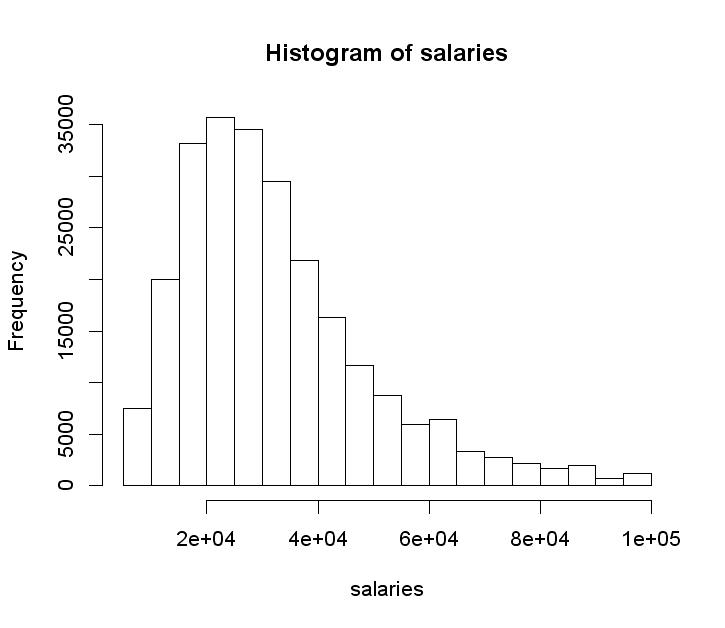
\includegraphics[width=7cm]{salaries_histogram.png}
            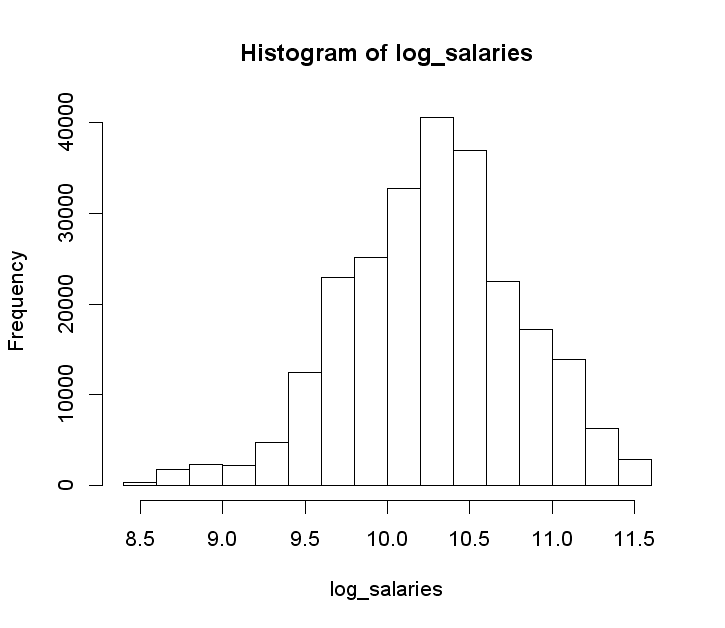
\includegraphics[width=7cm]{log_salaries_histogram.png}
        \end{center}
        т.е. логарифм преобразовывает распределение зарплат к нормальному. Но к сожалению этот вариант не получилось правильно настроить.

    \newpage
    \section{Подбор параметров для Vowpal Wabbit}
        Функция потерь: -{}-loss\_function quantile
        
        n-грамм: -{}-ngram: лучший результат показал 2-грамм без пропусков
        
        Далее настраивались параметры шага градиентного спуска. Лучшие результаты:
        
            \indent\indent -{}-initial\_t 0.5: параметр улучшил скорость сходимости
        
            \indent\indent -{}-power\_t 0.3: параметр улучшил точность
        
            \indent\indent -l 600: параметр улучшил точность

        L1-регуляризатор: -{}-l1 0.00000005: увеличил точность метода

        Количество итераций: 200: сошелся за 188 шагов
        
        Количество битов в таблице признаков: -b 27
        
        Квадратичная зависимость: -q tc (t - title, c - category)

    \section{Обучение и тестирование}

        Обучение велось на первых 100000 элементах обучающей выборки и тестировалось на 60000 последних элементах. После каждого подбора параметров считалась ошибка и подбор происходил, пока ошибка уменьшается. Как только получили хороший результат, обучаемся на полных данных и получаем ответы для контрольной выборки. Убеждаемся, что в системе Kaggle все отлично и радуемся или увидев результат хуже, огорчаемся.

    \section{Обработка ответов}

        Из исходных данных можно заметить, что зарплаты заданы целыми числами, кратными 100. Следовательно ответ нужно так же нормировать. Концы зарплат, близких к 500, например принадлежащих интервалу 250-750, округлить до 500 и т.д. Также можно заметить, что нет зарплат очень больших (>100000) и очень маленьких (<13000). Их можно отсечь, т.е. приравнять порогу.

        P.S. Эту идею мне подсказали =). На самом деле, очень хорошая идея и более того рабочая!

    \newpage
    \section{Заключение}
        В итоге получаем подобные следующему данные:

            \indent\indent 50000 |title charter senior quantiti surveyor |fulldescr award win multi disciplinari consult look experienc mric fric senior quantiti surveyor join success grow quantiti survey team this excel opportun experienc charter quantiti surveyor take team manag respons whilst maintain hand involv provid grow quantiti survey team south west area you high involv busi develop work alongsid director cost relat project you manag small team quantiti surveyor mentor apc junior quantiti surveyor guid charter qs varieti project pre contract post contract the success candid need charter mric fric senior quantiti surveyor consult experi you need client face senior quantiti surveyor proven track record busi develop experi grow qs divis candid must dynam ambiti enthusiast good interperson busi develop skill you need broad rang sector experi proven consult experi deliv project educ offic retail commerci sector some experi work hous associ sector would advantag essenti if feel relev experi would like discuss fantast opportun detail pleas call lee faux appli onlin email |loc somerset |category consult job

        следующую команду для обучения:

            \indent\indent vw -d train.txt -{}-passes 200 -{}-ngram 2 -k -c -f model.vw -{}-loss\_function quantile -l 600 -q tc -b 27 -{}-initial\_t 1 -{}-power\_t 0.3

        и следующую команду для получения ответов:

            \indent\indent vw -d test.txt -i model.vw -t -p predictions.txt

        В системе получаем 5067.83620 баллов на 31\% выборке и 5158.47037 баллов на 69\% выборке, выходим на 7 место и радуемся :)

\end{document}
